\section{Dualscattering approximation}
\label{sec_dualscattering}
%Summarize introduction

Multiple scattering is a key factor in the realistic rendering of hair, especially for dense light colored hair volumes (such as blond hair). The relative amount of absorption by light colored hair types is fairly low, so this means that light undergoes many scattering interactions inside the hair volume before the contribution is reduced to an amount that can be neglegible. The high geometric complexity of hair models coupled with the compexity of the light interaction in hair volumes makes computing the multiple scattering effect difficult~\cite{zinke}. Difficult to an extent that path-tracing is not a feasible solution, because it requires too much time and too many samples to reduce the noise and come to an acceptible rendering.

The dual scattering approximation, proposed by Zinke et al.~\cite{zinke} splits the multiple scattering computation in two components: global multiple scattering and local multiple scattering. The global multiple scattering component aims to compute the light traveling through the hair volume and reaching the neighborhood of the point of interest, while local multiple scattering accounts for the scattering events within this neighborhood~\cite{zinke}.

%
%Start from general rendering equation
%

Starting from the general rendering equation (see equation~\ref{rendering_eq}) and taking the diameter $D$ as being 1, we obtain the following equation.

\begin{equation}
L_o(x, \omega_o) = \int_{\Omega} L_i(x, \omega_i) S(\omega_i, \omega_o) \cos \theta_i d\omega_i
\end{equation}

This can be interpreted as the radiance in outgoing direction $\omega_o$ at a position $x$, equals the integral around the sphere ($\Omega$) of incident directions $\omega_i$ multiplied by the BSDF factor. The integration is a recursive process, and to find the incident radiance $L(x, \omega_i)$, another integration is needed from another point $x'$ to find $L_o(x', -\omega_i)$. The dualscattering approximation simplifies this process by defining the incident radiance as

\begin{equation}
L_i(x, \omega_i) = \int_{\Omega} L_d(\omega_d) \Psi(x, \omega_d, \omega_i) d\omega_d
\end{equation}

where $L_d$ is the incident radiance from outside the hair volume from direction $\omega_d$ (assuming distant illumination), and $\Psi(x, \omega_d, \omega_i)$ is the multiple scattering function denoting the fraction of light entering the hair volume from direction $\omega_d$ that is scattered inside the hair volume and finally arriving at point $x$ from direction $\omega_i$~\cite{zinke}. This works similar as to how subsurface scattering is defined.


%
%Reformulate equation practical for our situation
%

The main concept behind the dual scattering method is to approximate the multiple scattering function as a combination of two components. The global multiple scattering function $\Psi^G$ is used to compute the irradiance arriving at the neighborhood of point $x$ inside the hair volume, and the local multiple scattering function $\Psi^L$ approximates the multiple scattering of this irradiance within the local neighborhood of $x$~\cite{zinke}.
This results in the following equation, central to the dual scattering approximation model.

\begin{equation}
\Psi(x, \omega_d, \omega_i) = \Psi^G(x, \omega_d, \omega_i) (1 + \Psi^L(x, \omega_d, \omega_i))
\end{equation}

The global multiple scattering is thus responsible for gathering the irradiance from outside the hair volume and taking into account the scattering effects in the hair volume, to deliver an approximate amount of irradiance arriving at point $x$. It is important to see that the global multiple scattering removes the need to do extensive path tracing through the hair volume.

The local multiple scattering is more in line with the Marschner model: given the irradiance at point $x$, calculate the scattering effect of the local neighbourhood. For a neighborhood consisting of a single fiber, it boils down to evaluation of the Marschner model.

\subsection{Global multiple scattering function $\Psi^G$}

The global multiple scattering function $\Psi^G$ gathers the irradiance from outside the hair volume, approximating the amount of irradiance arriving at a point $x$ inside the hair volume. The global multiple scattering is defined as follows by Zinke et al.~\cite{zinke}:

\begin{equation}
\Psi^G(x, \omega_d, \omega_i) \approx T_f(x, \omega_d)\,S_f(x, \omega_d, \omega_i)
\end{equation}

The global multiple scattering $\Psi^G$ is the multiplication of forward transmittance $T_f$ and the average forward scattering spread $S_f$. The transmittance accounts for the amount of hairs in between the light source and the point to be shaded. The average forward scattering spread takes into account the loss of energy due to spreading of the light after each scattering event.

\subsubsection{Forward scattering transmittance}

In this thesis the forward scattering transmittance is computed by using a combination of ray shooting together with a voxel grid. Before rendering, a voxel grid is generated based on the hair model. Each voxel cell contains the density of the hairs in question. This is computed by traversing each hair fiber and storing the distance of the hair fiber segment in the voxel cell. In this way, cells that contain a lot of hair fibers, do have a higher density value.

When finding the irradiance at a position $x$ in direction $\omega_i$, a ray is shot in the direction of the light source. This ray is linearly ray-marched and for each position along the ray, the density value is looked up in the voxel cell. In this way, the global density value is computed for a specific direction $\omega_i$. The density factor can then be translated to the number of hair strands, by dividing the density by the volume of a voxel cell. This results in $n$, the number of hair strands in between the shading point $x$ and the light from direction $\omega_i$.

The forward scattering transmittance for the dual scattering method~\cite{zinke} is defined as follows:

\begin{equation}
T_f(x, \omega_d) = d_f(x, \omega_d) \prod_{k=1}^{n} a_f(\theta_d^k)
\label{dualscattering_Tf}
\end{equation}

where $d_f$ is the forward scattering density factor, which is a constant between $[0, 1]$ and usually set to $0.7$. This factor is a tweaking variable that can be changed dependent on the denseness of a hair volume. See figure~\ref{fig_df}.

\begin{figure}[h]
\begin{center}
\includegraphics[scale=0.2]{relatedwork/dualscattering_df.png}
\end{center}
\caption{This picture shows the cross section of a hair cluster. The factor $d_f$ is a tweaking variable to account for the portion of multiple scattered radiance reaching the point $x$. The orange region shows the forward scattering contribution. It can be seen that the light could have direct vision with point $x$ in which case there is no multiple scattered radiance. $d_f$ accounts for this fact. If $d_f$ is 1, then it is assumed that point $x$ is fully covered by hair strands as seen from the light direction. The same applies for the backward scattering attenuation factor $d_b$ (blue region). Usually both $d_f$ and $d_b$ are constant for the full model and set to 0.7.}
\label{fig_df}
\end{figure}


$a_f(\theta_d^k)$ is the average forward scattering attenuation at the $k$-th scattering event, which is computed in a precomputation step by integrating over all possible directions in the hemisphere and averaging the amount of forward scattered radiance. See the dual scattering method for more details~\cite{zinke} or the efficient implementation of the dual scattering model in RenderMan by Sadeghi and Tamstorf~\cite{sadeghi} for a more hands on approach.

In this work, a simplification is used by usng a constant orientation for all $k$ scattering events, under the assumption that we are dealing with human hair fibers that are locally similar in orientation. This means equation~\ref{dualscattering_Tf} can be simplified to the following equation.

\begin{equation}
T_f(x, \omega_d) = d_f(x, \omega_d) a_f(\theta_d)^n
\label{forwardscattering}
\end{equation}

\subsubsection{Forward scattering spread}

The spread function approximates the final angular distribution of front scattering light to find the probability of radiance coming to the point $x$ from direction $\omega_i$~\cite{zinke}. Because of the wide azimuthal scattering property of hair fibers, front scattered radiance quickly becomes isotropic in the azimuthal direction after only a few scattering events. For longitudinal scattering front scattered light is still anisotropic. The spread function is therefore split up into an isotropic azimuthal component ($1/\pi$) and an anisotropic longitudinal component described by a gaussian function $g$.

\begin{equation}
\label{dualscattering_Sf}
S_f(x, \omega_d, \omega_i) = \frac{s_f(\phi_d, \phi_i)}{\cos \theta_d} g(\theta_d + \theta_i, \sigma_f^2(x, \omega_d))
\end{equation}

where $s_f$ is $1/\pi$ for forward scattering directions and zero for backward scattering. $\sigma_f^2(x, \omega_d)$ is the total variance of forward scattering in the longitudinal direction. This is defined by the Marschner model as the squared standard deviation $\beta^2$ and is dependent on the longitudinal angle. Simplifying again by taking a constant $\theta_d$ gives us a single multiplication of number of hair strands multiplied by the longitudinal variance.

\begin{equation}
\sigma_f^2(x, \omega_d) = \sum_{k=1}^{n} \beta_f^2(\theta_d^k) \approx n \cdot \beta_f^2(\theta_d)
\end{equation}


\subsection{Local multiple scattering}

The local multiple scattering function $\Psi^L$ accounts for the multiple scattering events within the neighborhood of the point $x$. Since light paths that go through only forward scattering are included in the global multiple scattering function, light paths of the local multiple scattering function must include at least one backward scattering.

Because of backward scattering, the local multiple scattering is mostly smooth with subtle changes over the hair volume~\cite{zinke}.

The dual scattering model the local multiple scattering and the BCSDF of the hair fibers, approximating the result with a density factor $d_b$ and backscattering function.

\begin{equation}
\Psi^L(x, \omega_d, \omega_i) f_s(\omega_i, \omega_o) \approx d_b(x, \omega_d) f_{\textnormal{back}}(\omega_i, \omega_o)
\end{equation}

The density factor $d_b$ is a constant in the range $[0, 1]$, usually set to 0.7 approximating the density of the hair volume. The denser the hair, the stronger the backscattering event contributes to the result.

The backscattering is approximated with a material function $f_{back}$

\begin{equation}
f_{\textnormal{back}}(\omega_i, \omega_o) = \frac{2}{\cos \theta_d}A_b(\theta_d) S_b(\omega_i, \omega_o)
\end{equation}

\subsubsection{Average backscattering attenuation}

The average backscattering attenuation takes into account the attenuation in the local neighborhood of a point $x$. Since the global multiple scattering component already takes into account the forward scattering (meaning no backscatter events), we only need to deal with at least one backscatter event. Light coming from a light source, passing through the fiber at point $x$, needs an odd number of backscattering events for light to travel back to point $x$. The even number of backscattering events are ignored, since they are not directed to point $x$. Also, the dual scattering method ignores the contribution for more than three backscattering events, because their contribution becomes negligible low to the rendering result. 

If we denote $a_b(\theta_d)$ as the average backscattering attenuation and $a_f(\theta_d)$ as the average forward scattering attenuation (described in the previous section), then the average backscattering for a single backscattering event $A_1$ can be computed as the attenuation of a single backscatter event, multiplied by the sum of the infinite series of forward scattering attenuations. The same holds for the average backscattering attenuation for three backscattering events $A_3$, but now the possible paths are not a single sum anymore, but multiple sums to obtain the permutation of possible paths, dependent on where the backscattering event occurs in the sequence of forward scattering attenuations.

\begin{align}
A_1(\theta_d) &= a_b \sum_{i=1}^{\infty} a_f^{2i} = \frac{a_b a_f^2}{1 - a_f^2} \\
A_3(\theta_d) &= a_b^3 \sum_{i=1}^{\infty}  \sum_{j=0}^{i-1} \sum_{k=j+1}^{\infty} a_f^{2(i-j-1+k)} = \frac{a_b^3 a_f^2}{(1 - a_f^2)^3} \\
A_b(\theta_d) &= A_1(\theta_d) + A_3(\theta_d)
\label{avg_backscatter_series}
\end{align}

where $A_b$ is the average backscattering attenuation for 1 and 3 backscattering events. Figure~\ref{avg_backscatter_attenuation} provides a graphics representation of the backscattering events and how they are directed with respect to position $x$.

\begin{figure}
    \begin{tabular}{c}
    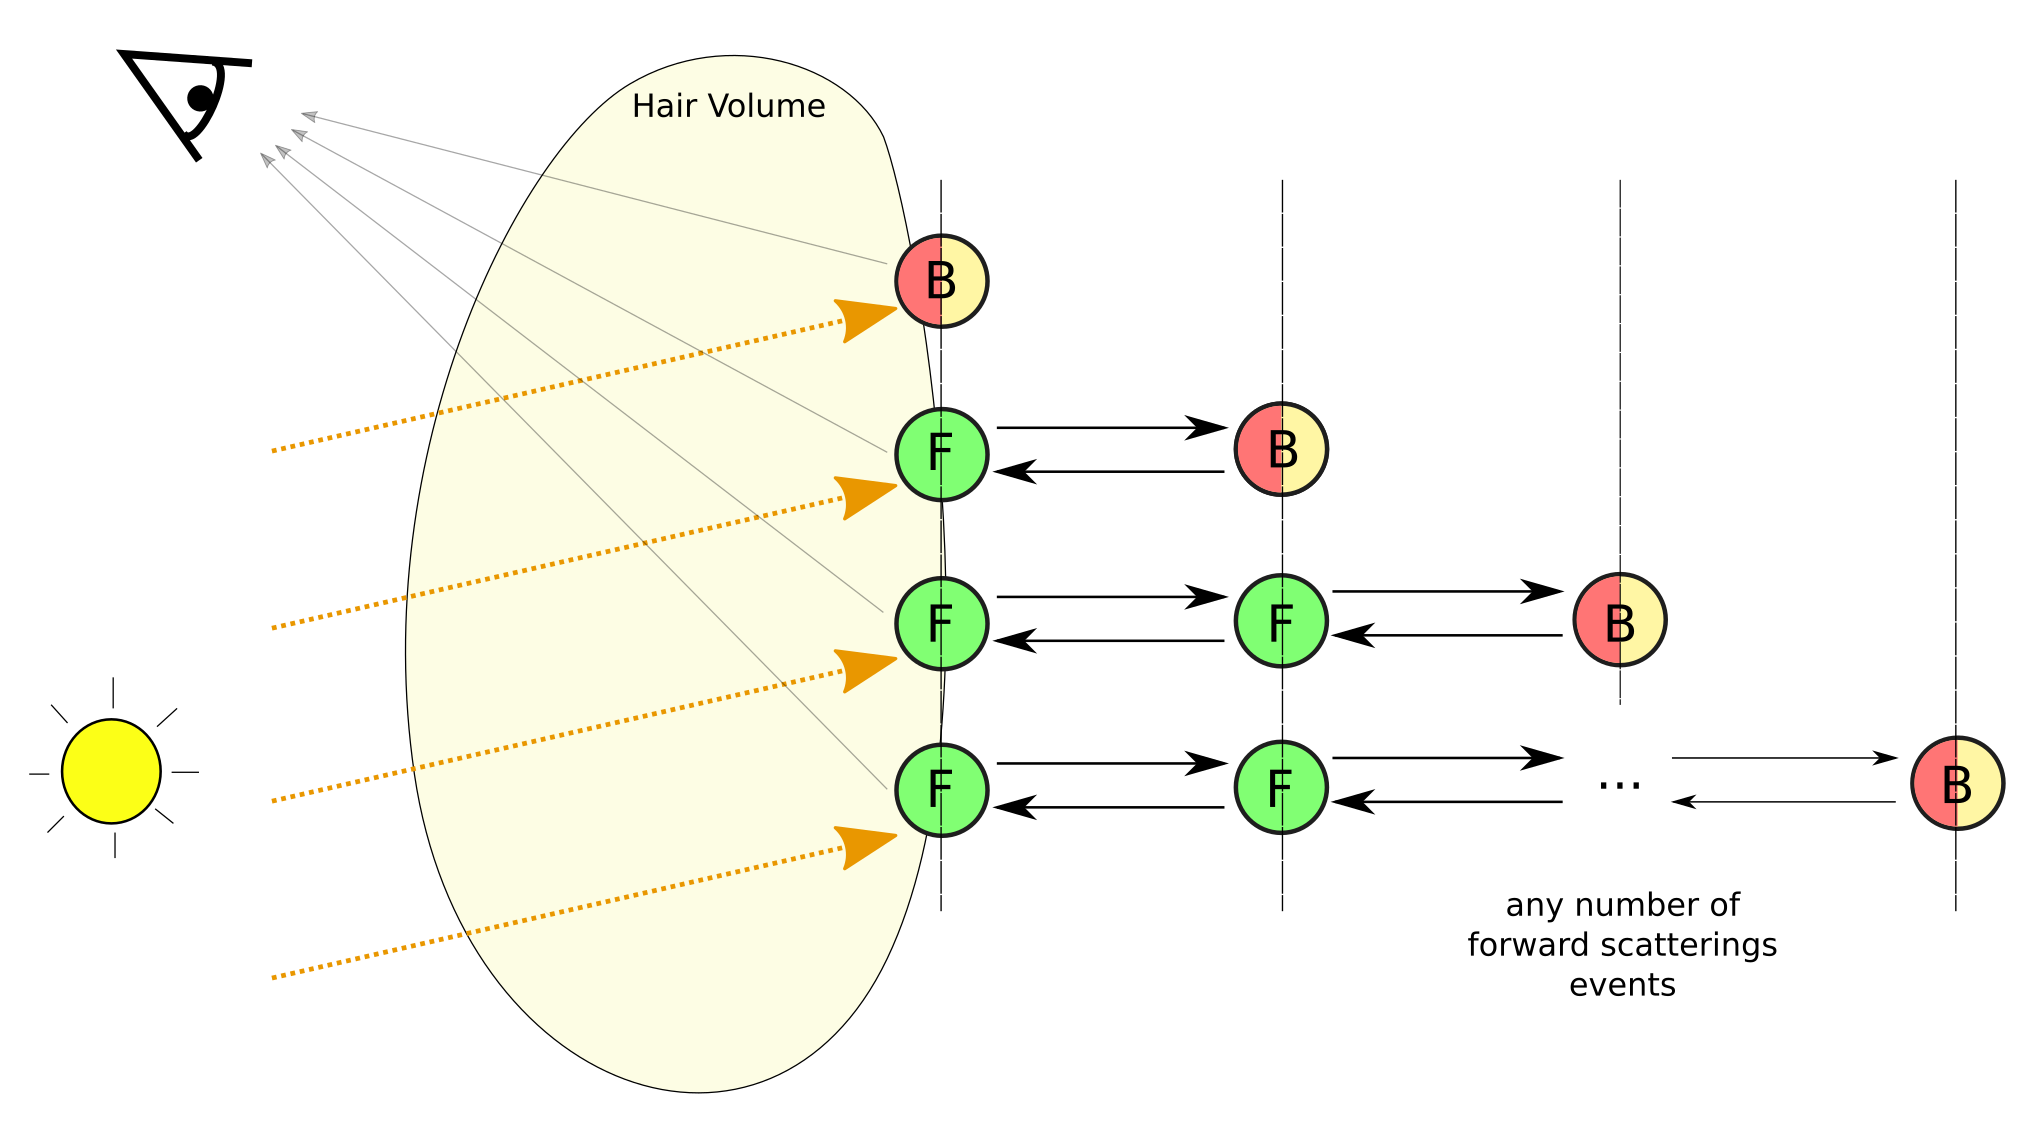
\includegraphics[scale=0.25]{avg_backscatter_1.png} \\
    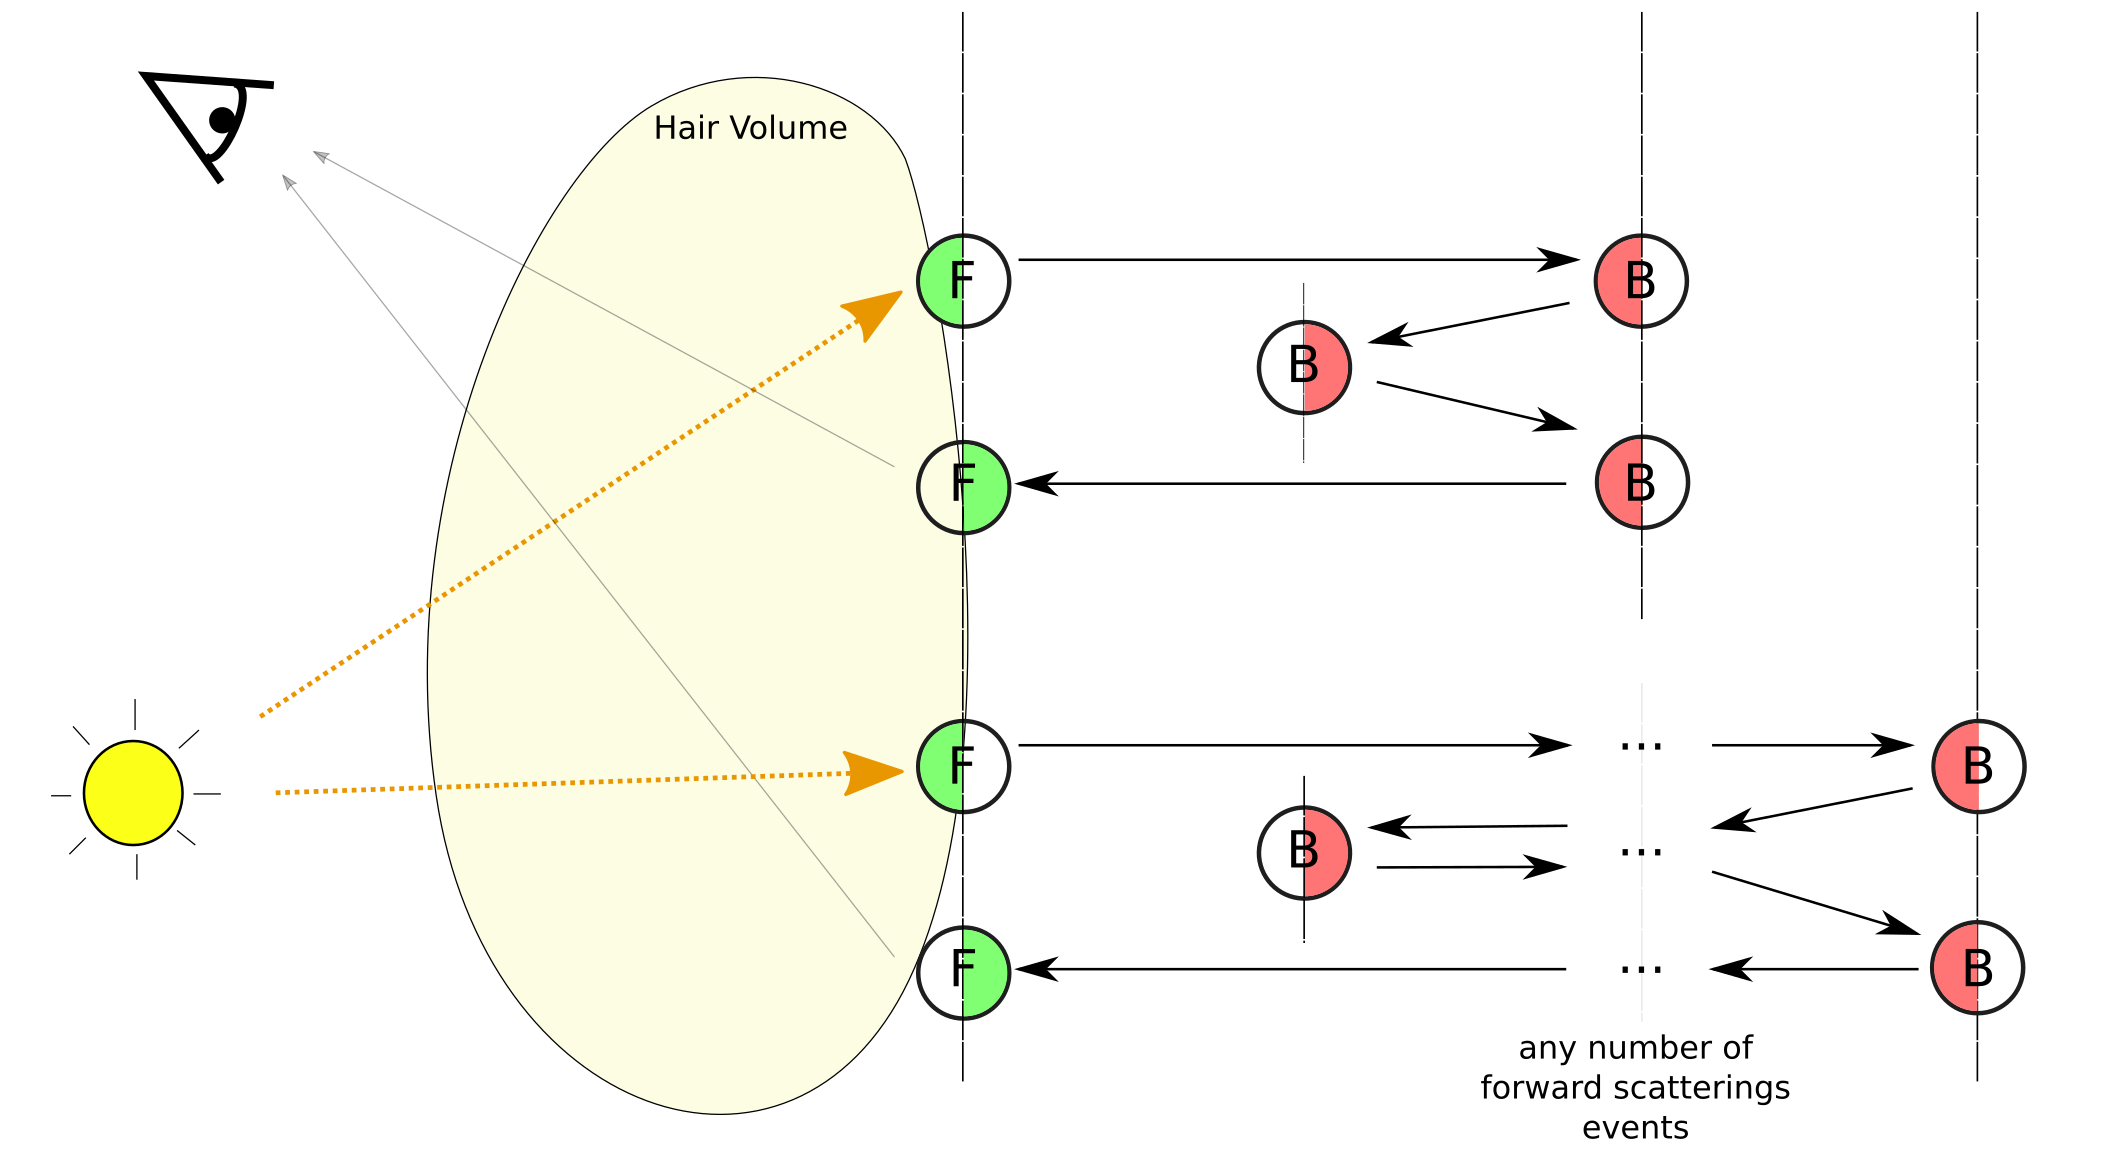
\includegraphics[scale=0.25]{avg_backscatter_3.png}
    \end{tabular}
    \caption{Visualization of the average backscattering attenuation $A_b$. The circles represent the cross section of the hair fibers. The color coded half circles represent the scattering event taking place, with red being a backward scattering event and green a forward scattering event, also indicated by B and F respectively. The orange ray correspond to the incident light from the light source. It represent the global illumination passing through the hair volume reaching the local neighborhood. The dual scattering method takes into account only one or three backscatter events. All permutations of one backscatter event ($A_1(\theta)$) is displayed in the top figure and all permutations for three backscatter events ($A_3(\theta)$) is displayed in the bottom figure. It is clear to see that the amount of
    forward scattering events may go to infinity, but that the amount of backscattering events is limited to one or three. This leads to the infinite series that can be written as shown in equation~\ref{avg_backscatter_series}.}
    \label{avg_backscatter_attenuation}
\end{figure}

\subsubsection{Average backscattering spread}

The average backscattering spread takes into account the loss of intensity, due to spreading of the light after backscattering events occur. This is similar to forward scattering events. The dual scattering method~\cite{zinke} presents the average backscattering spread $S_b(\omega_i, \omega_o)$ as

\begin{equation}
S_b(\omega_i, \omega_o) = \frac{s_b(\phi_i, \phi_o)}{\cos \theta} g(\theta_o + \theta_i - \Delta_b(\theta_d), \sigma_b^2(\theta_d)
\end{equation}

where $s_b$ equals $1/\pi$ for backward scattering directions and zero for forward scattering, $\Delta_b(\theta_d)$ is the average longitudinal shift caused by the scattering events.

The spread is modeled as a single gaussian function. It is important to notice that $\Delta_b$ represents the average mean and $\sigma^2$ represents the average variance, thereby taking into account the multitude of possible forward and backward scattering events.

The average longitudinal shift $\Delta_b$ and average longitudinal standard deviation $\sigma_b$ for backscattering can be precomputed by averaging over all directions. See the dual scattering method~\cite{zinke} for more details and ~\cite{sadeghi} for a more hands on approach.






